\documentclass[usenatbib]{mnras}
\usepackage{siunitx}
\usepackage{graphicx}	% Including figure files
\usepackage[mathletters]{ucs}
\usepackage[utf8x]{inputenc}
\usepackage[english]{babel}
\usepackage{float}
\usepackage{amssymb, amsmath, yhmath}

\bibliographystyle{apa}
\setlength{\bibhang}{1in}
\setcitestyle{authoryear, open={(},close={)}}
\renewcommand{\bibsection}{\section*{References}}

\usepackage{graphicx}

\newcommand{\squote}[1]{\lq #1\rq}

\renewcommand{\d}[1]{\ensuremath{\operatorname{d}\!{#1}}}
\newcommand{\poweV}[1]{\SI{e#1}{\electronvolt}}
\newcommand{\ineV}[2]{\SI{#1 e #2}{\electronvolt}}
\newcommand{\lcdm}{$\Lambda$CDM}
\DeclareSIUnit\parsec{pc}
\DeclareSIUnit\lightyear{ly}
\DeclareSIUnit\year{yr}
\usepackage{graphicx}
\begin{document}

\title[Substructure Dynamics]{On the continuous symmetry breaking of topologically nontrivial gauge invariant zesty heterotic p-adic maximal D = 9 SUGRAs defined over projective schemes: a meme-theoretic approach.}
\author[EDD]{
E\includegraphics[width = 0.4cm, height = 0.4cm]{B}ward \includegraphics[width = 0.4cm, height = 0.4cm]{B}itten$^{1}$ \thanks{Contact e-mail:}
\\
$^{1}$School of Natural Sciences, Institute for Advanced Study, Olden Lane, Princeton,
NJ 08540, USA}
\maketitle
\begin{abstract}
There is only one undeformed (i.e. ungauged, massless) maximal (i.e. N = 2) 9-dimensional supergravity (SUGRA). When defined over a complete scheme, which is projective if there is an ample, invertible sheaf on it, the SUGRA inherits a crunchy subalgebra whose cohomology can be refined by meme-theoretic methods on the stalks 
\end{abstract}

\begin{keywords}
cosmology: theory -- dark matter -- galaxies: structure
\end{keywords}

\section{Introduction}
	Overdense regions of dark matter collapse to roughly localized concentrations of matter called ‘halos’ which are well-described by spherically symmetric density profiles. However, compositionally identical halos may vary significantly from these profiles in small-scale power i.e. substructure. Simulations suggest that substructure forms clumps which are qualitatively similar to free dark matter halos. We adopt a substructure formalism which tracks subhalos as an estimate of total substructure. The secondary gravitational effects of these subhalos is dependent on the subhalo mass function and the shape of small halo profiles, which is directly dependent on properties of the dark matter physics under consideration.                
        The standard cosmological model (\lcdm) contains a massive electromagnetically non-interacting component known as Cold Dark Matter (CDM) with density parameter $\Omega_c = 0.259 \pm 0.006$. The properties of this substance are largely unknown and are assumed to be approximately that of a perfect fluid with negligible pressure compared to its energy density i.e. comprised of cold or non-relativistic matter. Constraints obtained from The Sloan Digital Sky Survey measurement of Ly-$\alpha$ forest power spectra and surveys of dwarf galaxies below the free-streaming scale rule out most models of relativistic (hot) matter as the primary component of dark matter \citep{can_neutrinos}. 
\par
        Although successful on cosmological scales, CDM models fail to make accurate predictions when compared with observations at distance scales less then \SI{10}{\kilo\parsec}. When compared with studies of dwarf galaxy rotation curves, CDM predicts unobserved density \squote{cusps} in the center of dark matter halos \citep{ultralight}. This failure is known as the \squote{cusp-core problem}. Another serious concern is the \squote{missing satellite problem}  \citep{missing_satellites}. The number of satellite galaxies predicted for a milky-way-like galaxy is greater than what we observe by an order of magnitude. This issue is sharpened by the \squote{too big to fail} problem of galaxy formation that claims some of the predicted satellites are so massive that it is impossible for them to not have any stars \citep{too_big_to_fail}. Various complex phenomena have been suggested as solutions to these problems such as baryonic feedback mechanisms which redistribute matter or  hypothetical dark matter self-interactions.

\par
	An alternative model gaining popularity known as Fuzzy Dark Matter (FDM) describes dark matter as comprised of ultra-light($m \approx \poweV{-22}$) bosons whose characteristic wavelength is on the order of $\SI{1}{\kilo\parsec}$. Such ultralight particles are possible in various theories beyond the standard model \citep{axion_cosmology}. In particular, the class of axion-like particles is a perfect candidate for FDM and therefore, we refer to the mass of the constituent particles of FDM as the axion mass $m_a$. Macroscopic quantum mechanical wave effects “smear” the density profile on scales less than $\sim \SI{1}{\kilo\parsec}$ which removes problematic cusps from the center of large halos. These cusps are replaced by dense self-gravitating quantum states known as soliton cores which may facilitate indirect observation evidence for FDM. Furthermore, the quantum mechanical pressure caused by the large wavelength of FDM suppresses the formation of low-mass halos and entirely eliminates the formation of any halo or subhalo smaller than this wavelength, reducing or eliminating the missing satellites problem. Significant further effort remains in determining further discrepancies between FDM and CDM and whether these can, in conjunction with observational constraints, rule out one or both of the models.
 
\par
        The dynamical effects of CDM have been studied in some detail, especially regarding the accretion and tidal stripping of CDM subhalos by large galaxies and their associated dark matter halos. On the other hand, research on the dynamics of FDM distributions is in its infancy. However, dynamical studies have focused on simulations which inherently have a fixed resolution and thus artificially suppress small-scale power. In this paper, we present analytic estimates for substructure dynamical fluctations which do not suffer from limited resolution. The resolution limit of simultations causes underestimates to subhalo populations and therefore to their dynamical effects. 
\par 
	CDM and FDM models predict significant differences in the distribution of halo substructure. The FDM subhalo mass function is zero below a cutoff scale determined by the axion mass expressed by the Jean’s scale at which quantum pressure and gravitational attraction balance:
\setlength{\belowdisplayskip}{4pt} \setlength{\belowdisplayshortskip}{4pt}
\setlength{\abovedisplayskip}{4pt} \setlength{\abovedisplayshortskip}{4pt}

\begin{equation}
k_J = 66.5 \cdot (1+z)^{1/4} \left( \frac{\Omega_a h^2}{0.12} \right) \left(\frac{m_a}{\poweV{-22}} \right)^{1/2} \si{\per\mega\parsec}
\end{equation}

as given by \citet{axion_cosmology}. \\ For light axions, the subhalo mass function is significantly suppressed though the entire range of substructure for a halo comparable to the Milky Way’s. However, FDM subhalos will exhibit solitons which, for moderately-sized subhalos and large axion masses, are very dense and largely unaffected by tidal disruption. In addition, a surprising standing wave phenomenon has been observed in the density profiles produced by small-scale FDM computer simulations \citep{cold_and_fuzzy}. These standing waves, named wavelets, radically alter the dark matter profile and may through gravitational interactions disturb the baryonic components in directly measurable ways. The primary effect of these wavelets is to introduce time-varying perturbations to the gravitational potential on a much shorter time-scale than the evolution of primary structure after the system has come into virial equilibrium. Follow-up work will investigate the magnitude of FDM wavelets compared with subhalo structure.  

\section{Modeling Substructure}
\subsection{Spatial Profile}
We model substructure as comprised entirely of subhalos which act as distinct massive particles subject only to gravitational attraction and tidal disruption. Following \citet{tidal_limit, unified_model} we adopt a
simplified model of CDM subhalo
formation and dynamics. The shape of
the subhalo mass function is assumed to
be spatially invariant, i.e. the position
and mass variables are decoupled. The
total density of subhalos is assumed to
follow the Navarro--Frenk--White (NFW) profile:
\begin{equation}
\rho(r) = \frac{\rho_0}{r/r_c (1+r/r_c)^2}
\end{equation} which also
describes the density profile of the
primary dark matter halo given by \citet{structure} from CDM simultations. This profile is fairly universal for the halos of massive cold particles which we assume accurately describe subhalos.

\subsection{Unresolved Mass Function}

	As the primary halo forms, it captures subhalos via accretion. The unresolved subhalo mass function refers to the distribution of subhalo masses at the time of accretion before dynmaical effects such as tidal stripping have biased the distribution. We assume the unresolved subhalo mass function is very close in shape to the free halo mass function truncated above the primary halo mass. Based on simulations given by \citet{dark_wave} we take this fraction to be $\sim 10\%$. The CDM halo mass function and corresponding subhalo mass function calculated from simultations \citep{pop_of_subhalos, unified_model} are well fit by a power law: 
\begin{equation}
\frac{\d{N}}{\d{\: \ln{m_{acc}}}} = A \left(\frac{m_{acc}}{M_p} \right)^{-p}
\end{equation}
with $p = 0.9$ and where $M_p$ is the mass of the primary or host halo. Unresolved CDM substructure is generated by sampling the distribution whose CDF is given by:
\begin{equation} \label{dist}
\mathbf{P}_{U;R}(u;r) = \frac{u^{-p} - u_{min}^{-p}}{u_{max}^{-p} - u_{min}^{-p}} \cdot \frac{\ln{(1+r/r_c)} - r/(r+r_c)}{\ln{(1+c)} - c/(1+c)} 
\end{equation}     
where $U = m_{acc}/M_p$ and $c = r_{max}/r_c$ is the concentration parameter. The normalization diverges as $m_{min} \to 0$ thus for numerical sampling trials a cutoff scale must be chosen. However, this divergence does not impose a minimum scale on our analytic results because it diverges slower than $1/m$ so the growth of perturbations due to small-scale structure is suppressed because they are proportional to the halo mass. The equivalent for FDM is calculated numerically via an equivalent process. The halo mass function is calcualted numerically from the Press--Schechter formalism \citep{substructure_FDM, marsh} and the soliton profile is fitted from simulations by \cite{schive_solitons}.

\subsection{Tidal Disruption} 
We adopt a simplistic model of tidal stripping which underestimates the total effect. A tidal radius is calculated by setting the tidal force on a test mass equal to the gravitational attraction of the subhalo. The resulting radius is:
\begin{equation}
R_t = R \left(\frac{m_{acc}}{2M_p(R)}\right)^{1/3} =  R_{max} \left(\frac{m_{acc}}{M_p}\right)^{1/3} f_T(R)
\end{equation} 
with $f_T(R) \propto R/R_c(\ln(1+R/R_c) - R/(R+R_c))^{-1/3}$ where $R_c$ is the core radius of the primary halo. We then suppose that total trucation occurs outside this radius and no disruption occurs within it. Thus,
\begin{equation}
\frac{m}{m_{acc}} = 
\begin{cases}
    \frac{\ln{(1+R_r/r_c)} - R_t/(r_c+R_t)}{\ln{(1+c)} - c/(1+c)},& \text{if } R_t < r_{max}\\
    1,              & \text{otherwise}
\end{cases}
\end{equation} 
However, $m_{acc} = 200 \rho_0 \frac{4}{3} \pi c(m)^3 r_c^3$ and $r_{max} = c(m) \: r_{c}$ so 
\begin{equation}
R_t = r_{max} f_T(R)
\end{equation}
\begin{equation} \label{trunc}
 \frac{m}{m_{acc}} = 
\begin{cases}
    \frac{\ln{(1 + x)} - x/(1 + x)}{\ln{(1+c)} - c/(1+c)},& \text{if } f_T(R) < 1\\
    1,              & \text{otherwise}
\end{cases}
\end{equation} where $x = c(m) \cdot f_T(R)$. Since $c$ is a weak function of $m$, the remaining mass fraction is also a weak function of $m$. Therefore, even the final resolved subhalo mass function is approximatly decoupled in mass and radius, in agreement with the results of \citet{unified_model}. Tidal disruption in the FDM case is similar, the density profile is truncated at the tidal radius. However, since the mass and radius of a soliton are inversely related \citep{solitons}, if the tidal radius is less than the soliton radius a runaway process will completely disrupt the halo. This is because as mass is stripped from the soliton, the soliton grows due to quantum pressure (previously halted by gravitational attraction) which pushes more mass outside the tidal radius. Due to the solitonic cores in FDM, the remaining mass fraction after tidal disruption is strongly dependent on the subhalo mass because the shape of the soliton profile and behavior are strongly mass-dependent. 

\section{calculating the dynamical influence of substructre}
\subsection{RMS Fluctuations}
Given a halo and a description of its substructure  we wish to determine its effects on the evolution of the system especially the baryonic compoents. The dynamics of the substructure introduce time-varying potentials which cause test particles to disperse in energy. This effect may contribute to the tickening of galactic disks and tidal streams. To assess magnitude of these effects we examine the time dependence of the potential. The root-mean-square (RMS) fluctuation at a given point in the halo is calculated as:
\begin{equation}
F_{RMS} = \sqrt{\left< \left( \frac{\d{\phi}}{\d{t}} \right)^2 \right>} = \sqrt{\left< \left(\sum_{i = 1}^N{\frac{M_i(r)G}{r_i^2} \hat{r} \cdot \vec{v}_i} \right)^2 \right>}
\end{equation}

	We assume that the velocities of distinct halos and their directional unit vectors are uncorrelated. Under these assumptions, the expected value is the sum of the expected value of each term:
\begin{align} \label{fluc}
F_{RMS} &= \sqrt{\sum_{i = 1}^N{\left< \left(\frac{M_i(r)G}{r_i^2}\right)^2 \right> \left< \left(\hat{r} \cdot \vec{v}_i \right)^2\right>}} \\ &= \sqrt{\sum_{i = 1}^N{\sigma(R) \left< \left(\frac{M_i(r)G}{r_i^2}\right)^2 \right>}} 
\end{align}  where $\sigma(R_i)$ is the linear velocity dispersion at the halo's position. This sum is estimated via numerical integration in python 2.7 with scipy v. 0.17.0 using the distribution of subhalo masses and positions given by equations (\ref{dist}, \ref{trunc}). 
 

\begin{figure}
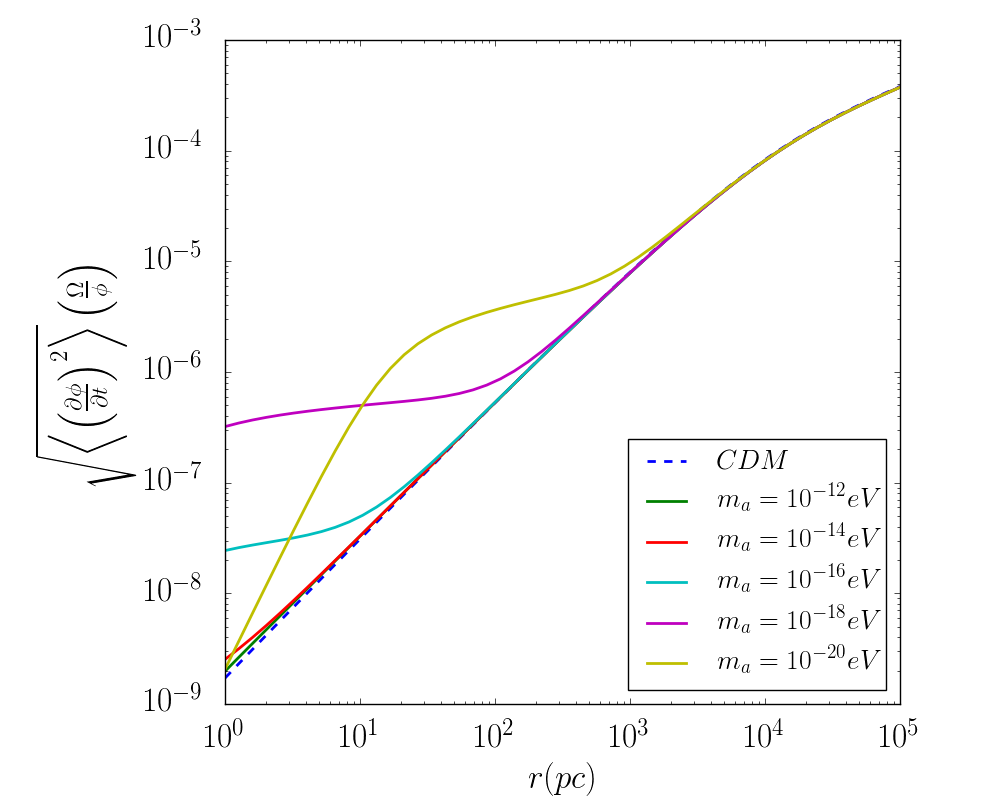
\includegraphics[width=\columnwidth]{High_Mass_Fluctuatations.png}
\vspace*{-5mm}
\caption{RMS fluctuations normalized to local host graviational potential and orbital period as a function of radius for various dark matter models with $m_a$ in the range \SIrange{e-12}{e-20}{\electronvolt}.}
\label{fig:highfluc}
\end{figure}

\begin{figure}
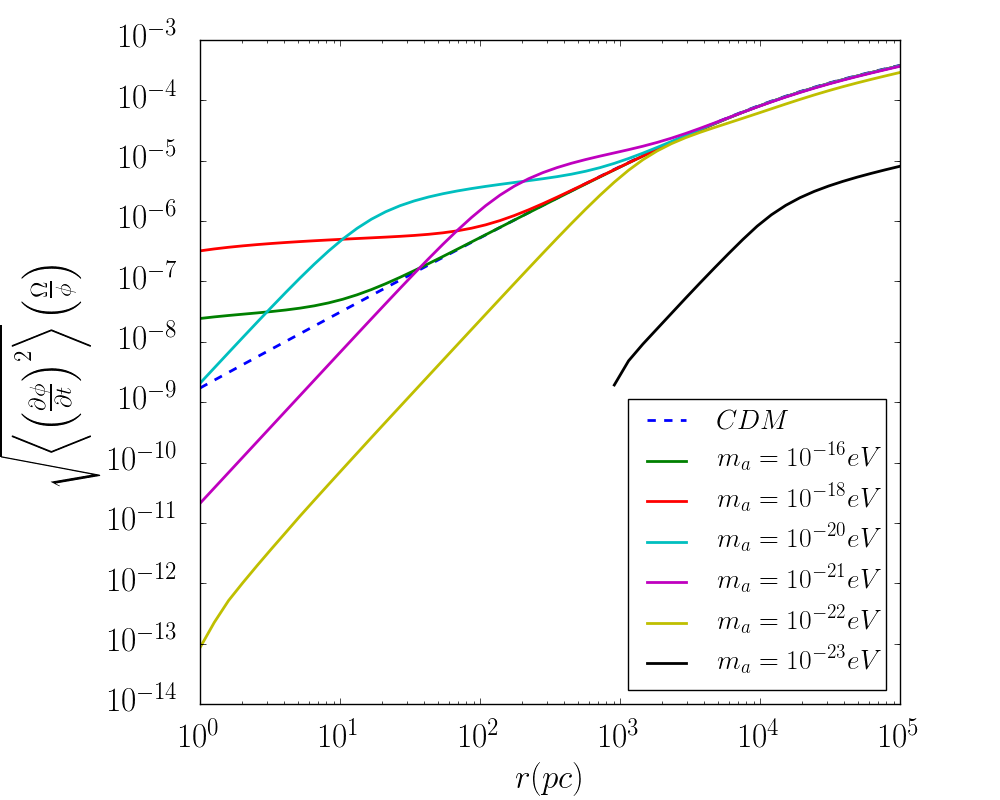
\includegraphics[width=\columnwidth]{Normed_Fluctuations.png}
\vspace*{-5mm}
\caption{RMS fluctuations normalized to local host graviational potential and orbital period as a function of radius for various dark matter models with $m_a$ in the range \SIrange{e-16}{e-23}{\electronvolt}.}
\label{fig:normfluc}
\end{figure}

\begin{figure}
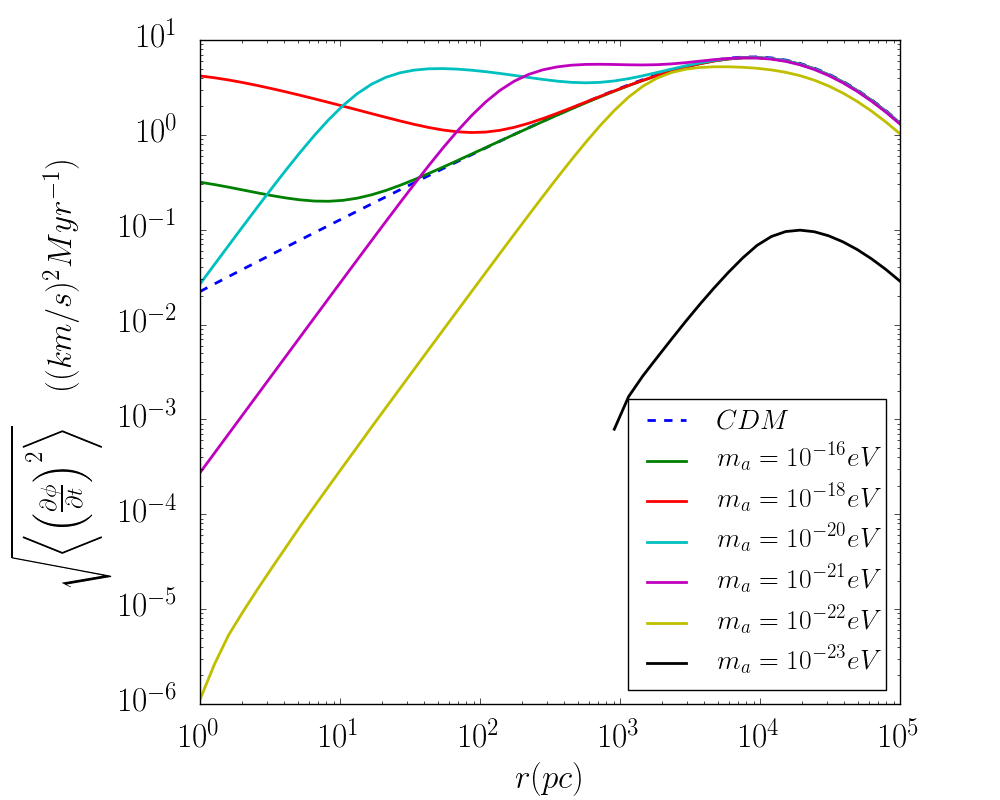
\includegraphics[width=\columnwidth]{Fluctuations.png}
\vspace*{-5mm}
\caption{Raw RMS fluctuations in \si{\kilo\metre\squared\per\second\squared\per\mega\year} as a function of radius for various dark matter models with $m_a$ in the range \SIrange{e-16}{e-23}{\electronvolt}.}
\label{fig:normfluc}
\end{figure}


\par
	In this paper, we present results for a halo with $M_p = 10^{12} M_{\odot}$ similar to the halo surrounding the Milky Way. Figure \ref{fig:highfluc} illustrates that for large axion masses, the FDM and CDM results are indistinguishable. This is an important consistency check of our calculations considering that CDM is the classical high-mass limit of FDM. However, as the mass of the axion increases, the fluctuations at small radii increase above their CDM counterpart. For a relativly heavy axion ($m_a > \poweV{-20}$), the suppression of small halos is insignificant and the solitons of subhalos are very dense, therefore the subhalos are less prone to tidal disruption. As the axion mass is further decreased, the number of small subhalos is significantly surpressed and the radius at which tidal effects completely disrupt solitons increases. For $m_a = \poweV{-23}$ all subhalos are completely tidally destroyed if $r < \SI{1}{\kilo\parsec}$ (see Figure \ref{fig:normfluc}). In the range \SIrange{e-16}{e-20}{\electronvolt}, FDM fluctations exceed those of CDM for a $10^{12} M_{\odot}$ primary halo. Lighter axions drastically reduce all fluctuations due to the suppression of small scale structure.  

\subsection{Fourier Power Spectrum}
We study the power spectrum of
the fluctuations in the gravitational
potential by approximating the path of each subhalo as a staight line over the interaction window. This approximation is only vaild for small fast-movivng subhalos but the orbital radii are large compared with the subhalo radii. Further study will improve this result. Under this approximation:
\begin{equation}
\tilde{\phi}(\omega) = \frac{1}{\sqrt{2\pi}}\int_{-\infty}^{\infty} \! \frac{M\left(\sqrt{b^2 + (vt)^2}\right)G}{\sqrt{b^2+(vt)^2}} e^{-i \omega t}\d{t}
\end{equation}
\\ \\

\begin{figure}
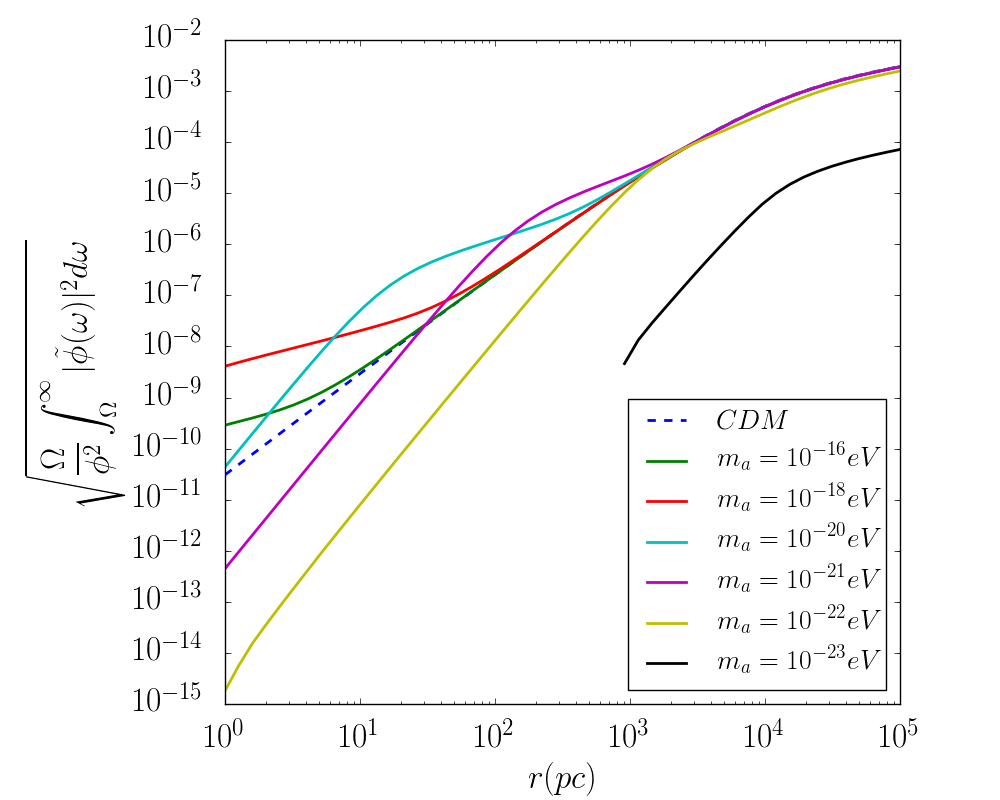
\includegraphics[width=\columnwidth]{Non-Adiabatic_Amplitude.png}
\vspace*{-5mm}
\caption{Non-adiabatic amplitude as a function of radius for various dark matter models with $m_a$ in the range \SIrange{e-16}{e-23}{\electronvolt}.}
\label{fig:fourierfluc}
\end{figure}

This integral is intractable when $b < r_{max}$ and must be computed numerically. However, when $b \geq r_{max}$,
\begin{equation}
\tilde{\phi}(\omega) = \frac{MG}{v} f_F\left(\frac{\omega b}{v} \right)
\end{equation} where
\begin{equation}
f_F(u) = \frac{1}{\sqrt{2\pi}} \int_{-\infty}^{\infty} \! \frac{e^{-iut'}}{\sqrt{1 + t'^2}} \d{t'} = \sqrt{\frac{2}{\pi}} K_0(u)
\end{equation}
Summing the power spectra of each halo,
we arrive at an approximate power
spectrum for the total fluctuations in
gravitational potential at a given point:
\begin{equation}
\left<\left| \tilde{\phi}(\omega) \right|^2 \right> = \left< \sum_{i = 1}^N \left(\frac{M_iG}{v_i} f_F\left(\frac{\omega b_i}{v_i} \right)\right)^2 \right>
\end{equation} 


The magnitude is normalized to the local
gravitational potential of the primary halo
and the frequency variable is normalized to
the local orbital period. This spectra is
summarized by integrating
over the power in high-frequency
(greater than orbital period) perturbations:
\begin{align}
P_{\Omega} &= \int_{\Omega}^{\infty} \! \left<\left| \tilde{\phi}(\omega) \right|^2 \right> \d{t} \\ &= \left< \sum_{i = 1}^N \left(\frac{M_iG}{v_i}\right)^2 \int_{\Omega_i}^{\infty} \! f_F\left(\frac{\omega b_i}{v_i} \right)^2 \d{\omega} \right> \\
&= \left< \sum_{i = 1}^N \left(\frac{M_iG}{v_i}\right)^2 \Omega_i \: F\! \left(\frac{\Omega b_i}{v_i} \right) \right>
\end{align} where 
\begin{equation}
F(u) = \frac{1}{u} \int_{u}^{\infty}\!\!\!\!\! f_F(x)^2 \d{x} = \frac{1}{u} \left[ G_{2, 4}^{3, 1} \left( \begin{smallmatrix} 1, \: \: 1 \\ \small\frac{1}{2}, \: \small\frac{1}{2}, \: \small\frac{1}{2}, \: 0 \end{smallmatrix} \Big| x, \: \frac{1}{2} \right) \right]^{\infty}_{u}
\end{equation}
$P_{\Omega}$ provides a measure of the total power in non-adiabatic perturbations which would
disperse orbiting test particles.


\subsection{Imposed Constraints}

We use the calculated gravitational potential to estimate the velocity dispersion caused by dynamical subhalos. An upper bound on the velocity dispersion due to subhalos is directly measurable by observing the distribution of velocities perpendicular to the disk of stars in the Milky Way. We provide an estimate of velocity dispersion by assuming that the gravitational perturbations at different times are independent. Therefore, test particles will undergo a random walk in velocity space whose total dispersion grows as:

\begin{align}
\frac{\d{ \Delta v^2}}{\d{t}} &= \frac{v_c^2}{t_c} &\qquad\text{thus}\qquad \Delta v &= v_c \left(\frac{t}{t_c}\right)^{\frac{1}{2}}
\end{align}
The characteristic velocity and time scale are estimated by assuming that the energy introduced to a test particle system by the fluctuating potential is shared evenly between kinetic and potential energy. This will overestimate the dispersion for slowly varying and spatially correlated fields. Future work in necessary to improve this estimate.


\begin{figure}
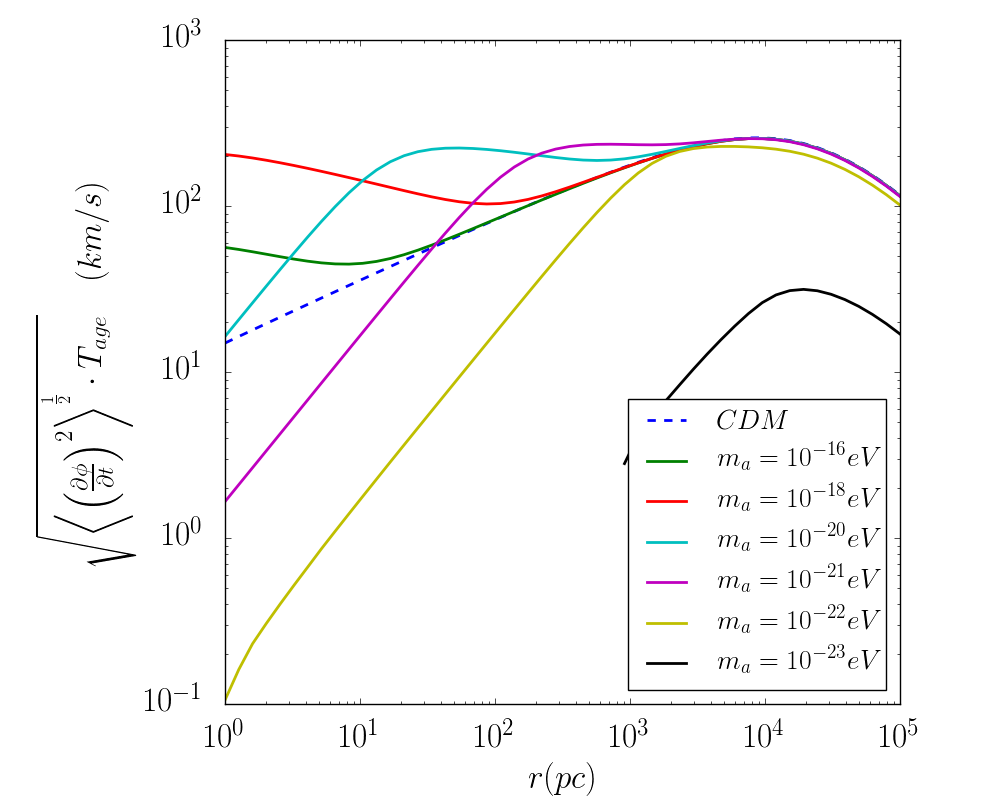
\includegraphics[width=\columnwidth]{Random_Walk_Velocity_Fluctation.png}
\vspace*{-5mm}
\caption{Velocity dispersion over the entire lifetime of the primary halo estimated from flucturations in the grviational potential plotted as a function of radius for various dark matter models with $m_a$ in the range \SIrange{e-16}{e-23}{\electronvolt}.}

\label{fig:fourierfluc}
\end{figure}
 
\par
The velocity dispersion mirrors behavior seen earlier in fluctuations. A very light axion will drastically reduce the velocity dispersion while a heavier axion will produce effects similar to those found in CDM. However, for a range of relatively heavy axions, FDM enhances estimated velocity dispersion above its counterpart CDM estimate at small radii. At its maximum, which, for a milky-way-like halo, occurs at $\sim \SI{10}{\kilo\parsec}$, CDM predicts in excess of \SI{100}{\kilo\meter\per\second} of velocity dispersion.
	
\par 

	The Milky Way has a thin disk of newer population I stars and a thick disk of older population II stars. The thick disk has velocity dispersion of approximately \SI{30}{\kilo\meter\per\second} in its thickest parts \citep{milky_way}. Therefore, no effect should produce more than \SI{30}{\kilo\meter\per\second} of velocity dispersion over the lifetime of the Milky Way. However, some of the heavier axion models of FDM and even CDM may give velocity dispersions that are above this threshold. To tell whether CDM exceeds this \SI{30}{\kilo\meter\per\second} threshold by a significant, margin we will need to do more detailed calculations. If these results are accurate, they support FDM over CDM because CDM will predict velocity dispersion in excess of bounds imposed by the Milky Way population II stars. Furthermore, they impose an upper bound on the mass of the FDM axion because FDM with an axion $m_a > \poweV{-21}$ predicts velocity dispersion in excess of even CDM predictions. However, an axion with $m_a < \poweV{-22}$ drastically suppresses the fluctuations from subhalos, mitigating this observational discrepancy. Further work is necessary to strengthen the precision and significance of this bound. Our efforts focus on verifying these results with Monte Carlo simulations which will include variability between subhalo profiles. More detailed calculations will incorporate increased tidal disruption of halos with highly eccentric orbits.  Furthermore, FDM wavelets may provide another very important element of FDM substructure which we have not yet considered.


\section*{Acknowlegements}
We thank Mihir Kulakarni for his code to calculate the FDM halo mass function and his invaluable guidance on this project and Philip Mocz and Hsi-Yu Schive for helpful discussions about solitons and wavelets. We also thank Hsi-Yu Schive for providing simulation data. 

\bibliography{mybib}


 
\end{document}